\section{Overview}
In this chapter we will present in detail the planning and approach we followed to establish the studies and analyze their results. Two studies, a controlled one, followed by a non-controlled one were conducted with the participation of 9 undergraduate master's degree and third-year bachelor's degree students enrolled in the "Embedded Systems" course at the University of Salerno in Italy. Participation in the studies was agreed upon by the students and was voluntary.

Before taking part in the first study, a set of lectures and training sessions was held with the objective of training the participants on the topics tackled by the studies, namely unit testing, test scaffolding and TDD.



\section{Research Questions}
The study we performed aimed at answering the following Research Questions (RQs):
\begin{itemize}
    \item \textbf{RQ1}: Are there differences between the application TDD and NO-TDD in the external quality of the implemented solutions, developers' productivity, and number of test cases written?
    \item \textbf{RQ2}: (può essere unita alla precedente?) Are there differences between TDD and NO-TDD in (cyclomatic and cognitive complexities, lines of code and numbers code smells)
\end{itemize}

RQ1 was defined to \dots



\section{Experimental Units}
The participants for these studies were students at the University of Salerno, in Italy; they were a mix of second-year master's degree students in Salerno, and students visiting the university by means of the Erasmus program; this last group was further made up of master's degree students and third-year bachelor's degree students. Both groups were enrolled in the Embedded Systems course at the University of Salerno.

The course covered the following topics: \dots but no TDD, which was in turn covered by the lectures and training sessions preceding the studies.

Participating in the studies was voluntary; the students were informed that any gathered data would be treated anonymously and shared for research purposes only; furthermore, participation would not directly affect their final mark for the Embedded System course; however, in order to encourage student participation, those who took part in the studies were rewarded with a bonus in their final mark. Among the students taking the course, 9 participated.

The participants for the tasks were asked to carry out their assignment by either using TDD or no-TDD (i.e., any approach they preferred, except for TDD) depending on the group they were partitioned in. and on the period the task took place.



\section{Experimental Materials}
The experimental objects for the studies were three code katas, programming exercises aimed at practicing a technique or a programming language:
\begin{itemize}
    \item \textbf{IntelligentOffice}:
    \item \textbf{CleaningRobot}:
    \item \textbf{SmartHome}:
\end{itemize}

Further details on the experimental objects, including user stories, hardware used, and other information, are provided as an appendix to this thesis.



\section{Variables}
Independent variables:
\begin{itemize}
    \item \textbf{Condition}: a nominal variable assuming two values, TDD and no-TDD.
    \item \textbf{Period}: the data was collected over two periods for the controlled study, and over an additional period for the non-controlled study. During the three periods both treatments (TDD or no-TDD) were applied.
    \item \textbf{Group}: variable representing the two groups. It can assume the values G1 and G2.
\end{itemize}


As for the dependent variables considered in the studies, these are: \textbf{QLTY}, \textbf{PROD}, \textbf{TEST}, \textbf{CYC}, \textbf{COG}, \textbf{LOC}.
The variables QLTY, PROD and TEST have been used in previous empirical studies \cite{DBLP:journals/tse/ErdogmusMT05}, \cite{DBLP:journals/tse/FucciETOJ17}, \cite{DBLP:journals/ese/TosunDFVTESOTJJ17}. As for the others, \dots

QLTY quantifies the external quality of the solution a participant implemented. It is formally defined as follows: 
\[
    QLTY = \frac{\sum_{i=1}^{\#TUS} QLTY_i}{\#TUS} * 100 
\]
where $\#TUS$ is the number of user stories a participant tackled, while $QLTY_i$ is the external quality of the $i-th$ user story; to determine whether a user story was tackled or not, the asserts in the test suite corresponding to the story were checked: if at least one assert in the test suite for the story passed, than the story was considered as tackled. $\#TUS$ is formally defined as follows:
\[
    \#TUS = \sum_{i=1}^{n} 
        \begin{cases}
            1 & \text{$\#ASSERT_i(PASS) > 0$}\\
                0 & \text{otherwise}
        \end{cases}
\]
Finally, the quality of the $i-th$ user story (i.e., $QLTY_i$) is defined as the ratio of asserts passed for the acceptance suite of the $i-th$ user story over the total number of asserts in the acceptance suite for the same story. More formally:
\[
    QLTY_i = \frac{\#ASSERT_i(PASS)}{\#ASSERT_i(ALL)}
\]

PROD estimates the productivity of a participant. It is computed as follows:
\[
    PROD = \frac{\#ASSERT(PASS)}{\#ASSERT(ALL)} * 100
\]
where $ASSERT(PASS)$ is the total number of asserts that have passed, by considering all acceptance test suites, while $ASSERT(ALL)$ refers to the total number of asserts in the acceptance suites. The $PROD$ variable can assume values between 0 and 100, where a value close to 0 indicates low productivity in the implemented solution, while a value close to 1 refers to high productivity.

The TEST variable quantifies the number of unit tests a participant wrote. It is defined as the number of assert statements in the test suite written by the participant; this variable ranges from 0 to $\infty$.


As for the additional three dependent variables regarding the general code quality in the submitted projects, these are defined as follows:
(\textbf{$CYC$}) refers to the Cyclomatic Complexity of the implemented solution; it is a value used to determine the stability and level of confidence in a program and it measures the number of linearly-independent paths inside a program module. A program with a lower Cyclomatic Complexity is generally easier to understand and less "risky" to modify; it can be used as an estimate on how difficult the code will be to cover/test.

(\textbf{$COG$}) is the Cognitive Complexity of the solution; it is a measurement of how difficult a program module is to intuitively understand. A method's Cognitive Complexity is based on a few rules \cite{CognitiveComplexity}:
\begin{enumerate}
    \item Code is not considered more complex when it uses shorthand syntax that the language provides for collapsing multiple statements into one.
    \item Code is considered more complex for each "break in the linear flow of the code".
    \item Code is considered more complex when "flow breaking structures are nested"
\end{enumerate}

Finally, $LOC$ is the total number of lines of code written by the participant; it's defined as the sum of the lines of code in both the production code and the test code.



\section{Study design}
The participants were randomly split into two groups, G1 and G2, having 4 and 5 participants respectively. For the first period P1, the group G1 was assigned the TDD task, while the group G2 was assigned the no-TDD task; on the other hand, during period P2, the group G1 was assigned the no-TDD task, while the group G2 was assigned the TDD task.
Therefore, the design of our study can be classified as a repeated-measures, within-subjects design. In each period, the participants in G1 and G2 dealt with different experimental objects. For instance, in P1, the participants in G1 dealt with BSK, while those in G2 with MRA. At the end of the study, every participant had tackled each experimental object only once.

\section{Procedure}
Before our study took place, we collected some demographic information on the participants. To this end, the participants were asked to fill out an on-line pre-questionnaire (created by means of Google Forms).

The Embedded Systems course, during which the study was conducted, started in September 2022. The first task, P1, took place on Tuesday, December 6th 2022, while the second, P2, took place on Tuesday, December 13th 2022.

Between the start of the course and P1, the participants had never dealt with TDD, while they were somewhat familiar with unit testing and iterative test-last development. In the weeks before P1, TDD was introduced to the participants via some lectures; also had taken part in ... training sessions on TDD and completed some homework by using this development practice.





\section{Results}
In this section we will report the values observed for each dependent variable.
Besides the tables, box plot charts will be used to visualize the values assumed by the dependent variables.
A box plot chart is a type of chart often used in explanatory data analysis; it visually shows the distribution of numerical data and skewness through displaying the data quartiles (or percentiles) and averages.

Box plot definitions:
\begin{itemize}
    \item \textbf{Minimum value}: the lowest value, excluding outliers (shown at the end of the lower whisker).
    \item \textbf{Maximum value}: the highest score, excluding outliers (shown at the end of the upper whisker).
    \item \textbf{Median}: marks the mid-point of the data and is shown by the line that divides the box into two parts. Half the values are greater than or equal to this value and half are less than this value.
    \item \textbf{Inter-quartile range}: The middle “box” represents the middle 50\% of values for the group. The range of values from lower to upper quartile is referred to as the inter-quartile range. The middle 50\% of scores fall within the inter-quartile range.
    \item \textbf{Upper quartile}: 75\% of the scores fall below the upper quartile.
    \item \textbf{Lower quartile}: 25\% of scores fall below the lower quartile.
    \item \textbf{Whiskers}: the upper and lower "whiskers" represent scores outside the middle 50\% (i.e. the lower 25\% of scores and the upper 25\% of scores).
    \item \textbf{Outliers}: observations that are numerically distant from the rest of the data. They are defined as data points that are located outside the whiskers of the box plot, and are represented by a dot.
\end{itemize}

\noindent To provide an example of the kind of information that a box plot chart can provide, please consider the following figure displaying four student groups' opinions on a subject:

\dots

Some observations that can be made include:
\begin{itemize}
    \item The box plot is comparatively short (see box plot  (2)). This suggests that overall the student have a high level of agreement and therefore the values are very similar between each other.
    \item The box plot is comparatively tall (see box plots (1) and (3)). This, on the other hand, suggests students hold quite different opinions about this aspect or sub-aspect.
    \item Obvious differences between box plots (see box plots (1) and (2), (1) and (3), or (2) and (4)). Any obvious difference between box plots for comparative groups is worthy of further investigation.
    \item The 4 sections of the box plot are uneven in size (see box plot (1)). This reveals that many students share a similar view at certain parts of the scale, but in other parts of the scale students are more variable in their views. A long upper whisker in the means that students views are varied among the most positive quartile group, and very similar for the least positive quartile group. 
    \item Same median, different distribution (see box plots (1), (2), and (3)). The medians, which generally tend to be close to the average, are at the same level. However, the box plots in these examples show very different distributions of views. It's always important to consider the pattern of the whole distribution of responses in a box plot.
\end{itemize}


\textbf{Boxplot da inserire appena smetto di litigare con le immagini in Latex. Per il momento sono in una cartella separata}

\noindent\textbf{Task 1}: The following tables display the values for the variables measured for the first experimental task, IntelligentOffice, for the two groups, by applying each of the two conditions.
\\ \  \\
\noindent
\begin{tabular}{ |p{2cm}||p{1.6cm}|p{1.6cm}|p{1.6cm}|p{1.6cm}|p{1.6cm}|p{1.6cm}| }
    \hline
        \multicolumn{6}{|c|}{Task 1 - TDD} \\
    \hline
        Metric & Min & Max & Mean & Median & Std \\
    \hline
        QLTY & 73 & 96 & 81.12 & 77.77 & 10.73 \\
        PROD & 72 & 96 & 83 & 82 & 10 \\
        TEST & 8 & 10 & 9.5 & 10 & 1 \\
        CYC & 21 & 28 & 24.75 & 25 & 2.87 \\
        COG & 14 & 25 & 19 & 18.5 & 4.69 \\
        LOC & 154 & 195 & 167 & 159.5 & 18.95 \\
    \hline
\end{tabular}
\\ \  \\
\noindent
\begin{tabular}{ |p{2cm}||p{1.6cm}|p{1.6cm}|p{1.6cm}|p{1.6cm}|p{1.6cm}|}
    \hline
        \multicolumn{6}{|c|}{Task 1 - NO-TDD} \\
    \hline
        Metric & Min & Max & Mean & Median & Std\\
    \hline
        QLTY & 65.55 & 82 & 75.35 & 78.77 & 7.43 \\
        PROD & 56 & 84 & 76 & 80 & 11.66 \\
        TEST & 0 & 12 & 3.8 & 0 & 5.49 \\
        CYC & 12 & 18 & 15.6 & 16 & 2.19 \\
        COG & 9 & 17 & 14 & 15 & 3 \\
        LOC & 74 & 157 & 111.6 & 100 & 33.69 \\
    \hline
\end{tabular}
\\ \  \\

\noindent \textbf{Task 2}: The following tables display the values for the variables measured for the second experimental task, CleaningRobot, for the two groups, by applying each of the two conditions.
\\ \  \\
\noindent
\begin{tabular}{ |p{2cm}||p{1.6cm}|p{1.6cm}|p{1.6cm}|p{1.6cm}|p{1.6cm}|}
    \hline
        \multicolumn{6}{|c|}{Task 2 - TDD} \\
    \hline
        Metric & Min & Max & Mean & Median & Std\\
    \hline
        QLTY & 0 & 100 & 74.44 & 100 & 43.31 \\
        PROD & 8 & 100 & 38.6 & 21 & 37.35 \\
        TEST & 0 & 13 & 5.4 & 3 & 5.12 \\
        CYC & 9 & 19 & 12 & 10 & 4.06 \\
        COG & 2 & 40 & 12.8 & 4.0 & 15.91 \\
        LOC & 80 & 203 & 128 & 115 & 45.61 \\
    \hline
\end{tabular}

\noindent
\begin{tabular}{ |p{2cm}||p{1.6cm}|p{1.6cm}|p{1.6cm}|p{1.6cm}|p{1.6cm}|}
    \hline
        \multicolumn{6}{|c|}{Task 2 - NO-TDD} \\
    \hline
        Metric & Min & Max & Mean & Median & Std\\
    \hline
        QLTY & 74 & 94.43 & 83.07 & 81.94 & 10.17 \\
        PROD & 52 & 73 & 60.5 & 58.5 & 10.24 \\
        TEST & 5 & 12 & 9 & 9.5 & 2.94 \\
        CYC & 16 & 36 & 23.5 & 21 & 9 \\
        COG & 11 & 49 & 29 & 28 & 15.57 \\
        LOC & 178 & 260 & 207.5 & 196 & 37.11 \\
    \hline
\end{tabular}
\\ \  \\

\textbf{Tasks 1 \& 2}: the following tables display the values for the variables measured for the first two experimental tasks, i.e., the controlled study, for the two groups, by applying each of the two conditions.
\\ \  \\
\noindent
\begin{tabular}{ |p{2cm}||p{1.6cm}|p{1.6cm}|p{1.6cm}|p{1.6cm}|p{1.6cm}|}
    \hline
        \multicolumn{6}{|c|}{Task 1 \& 2 - TDD} \\
    \hline
        Metric & Min & Max & Mean & Median & Std\\
    \hline
        QLTY & 0 & 100 & 77.41 & 82 & 31.52 \\
        PROD & 8 & 100 & 58.33 & 72 & 35.76 \\
        TEST & 0 & 13 & 7.22 & 8 & 4.26 \\
        CYC & 9 & 28 & 17.66 & 19 & 7.51 \\
        COG & 2 & 40 & 15.55 & 14 & 12.06 \\
        LOC & 80 & 203 & 145.33 & 154 & 39.97 \\
    \hline
\end{tabular}
\\ \  \\
\noindent
\begin{tabular}{ |p{2cm}||p{1.6cm}|p{1.6cm}|p{1.6cm}|p{1.6cm}|p{1.6cm}|}
    \hline
        \multicolumn{6}{|c|}{Task 1 \& 2 - NO-TDD} \\
    \hline
        Metric & Min & Max & Mean & Median & Std\\
    \hline
        QLTY & 65.55 & 94.43 & 78.78 & 78.77 & 9.11 \\
        PROD & 52 & 84 & 69.11 & 73 & 13.22 \\
        TEST & 0 & 12 & 6.11 & 7.0 & 5.08 \\
        CYC & 12 & 36 & 19.11 & 16 & 7.07 \\
        COG & 9 & 49 & 20.66 & 15 & 12.56 \\
        LOC & 74 & 260 & 154.22 & 157 & 60.32 \\
    \hline
\end{tabular}
\\ \  \\


\textbf{Tasks 3}: finally, these last tables display the values for the variables measured for the third experimental task (non-controlled study), SmartHome, for the two groups, by applying each of the two conditions.
\\ \  \\
\noindent
\begin{tabular}{ |p{2cm}||p{1.6cm}|p{1.6cm}|p{1.6cm}|p{1.6cm}|p{1.6cm}|}
    \hline
        \multicolumn{6}{|c|}{Task 3 - TDD} \\
    \hline
        Metric & Min & Max & Mean & Median & Std\\
    \hline
        QLTY & 85 & 100 & 95 & 100 & 7.07 \\
        PROD & 83.33 & 100 & 93.33 & 100 & 9.13 \\
        TEST & 7 & 18 & 11.6 & 12 & 4.15 \\
        CYC & 15 & 30 & 22.6 & 20 & 6.58 \\
        COG & 18 & 34 & 25.8 & 25 & 7.08 \\
        LOC & 150 & 232 & 187 & 175 & 36.15 \\
    \hline
\end{tabular}
\\ \  \\
\noindent
\begin{tabular}{ |p{2cm}||p{1.6cm}|p{1.6cm}|p{1.6cm}|p{1.6cm}|p{1.6cm}|}
    \hline
        \multicolumn{6}{|c|}{Task 3 - NO-TDD} \\
    \hline
        Metric & Min & Max & Mean & Median & Std\\
    \hline
        QLTY & 80 & 100 & 86.25 & 82.5 & 9.46 \\
        PROD & 75 & 100 & 83.33 & 79.16 & 11.78 \\
        TEST & 0 & 11 & 4.5 & 3.5 & 5.44 \\
        CYC & 16 & 23 & 19.5 & 19.5 & 2.88 \\
        COG & 19 & 25 & 21 & 20 & 2.70 \\
        LOC & 93 & 164 & 125.5 & 122.5 & 36.82 \\
    \hline
\end{tabular}
\\ \  \\

\begin{figure}
    \centering
    \begin{subfigure}{.5\textwidth}
        \centering
        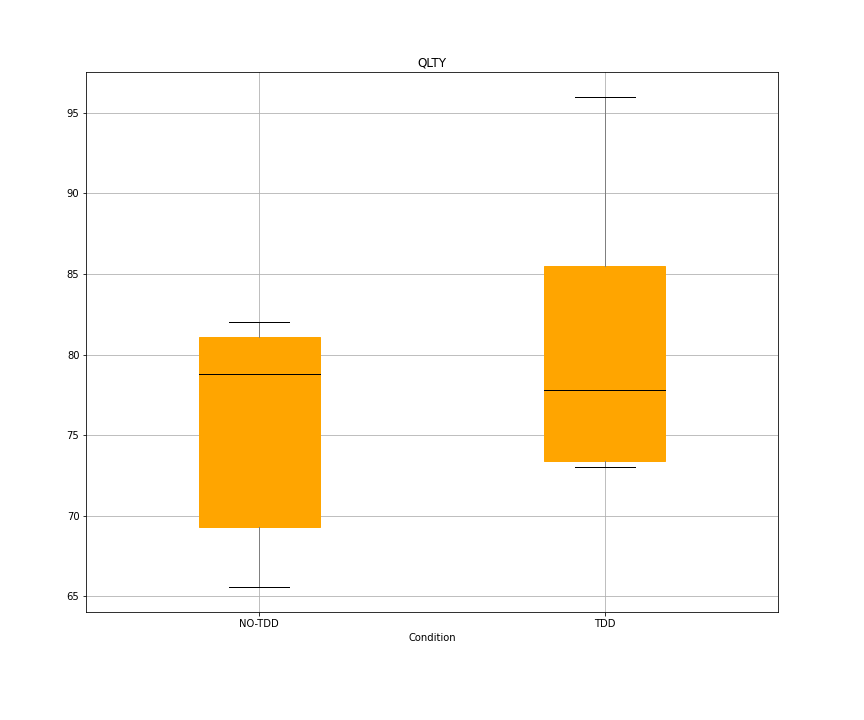
\includegraphics[width=.4\linewidth]{figures/box plots/task1/p1_condition_qlty_bp.png}
        \caption{A subfigure}
        \label{fig:sub1}
    \end{subfigure}%
    \begin{subfigure}{.5\textwidth}
        \centering
        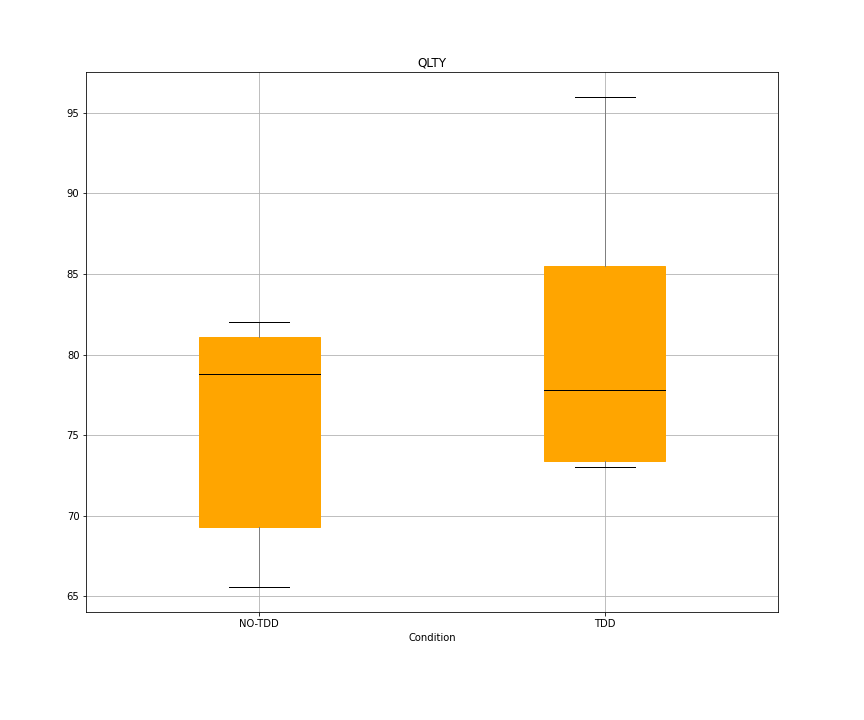
\includegraphics[width=.4\linewidth]{figures/box plots/task1/p1_condition_qlty_bp.png}
        \caption{A subfigure}
        \label{fig:sub2}
    \end{subfigure}
    \caption{A figure with two subfigures}
    \label{fig:test}
\end{figure}


\section{Discussion}
\subsection{Answers to Research Questions}


\subsection{Implications}


\subsection{Threats to Validity}